%%%%%%%%%%%%%%%%%%%%
%
% $Beschreibung: Momentenverlauf für den NEMA 17 $
% $Autor: Grönke $
% $Datum: 20.06.2024 $
% $Pfad: DemonstratorSchrittmotor/DeveloperDoc/tikz/MomentenverlaufSchrittmotor.tex $
% $Version: 1 $
%
%
%%%%%%%%%%%%%%%%%%%

	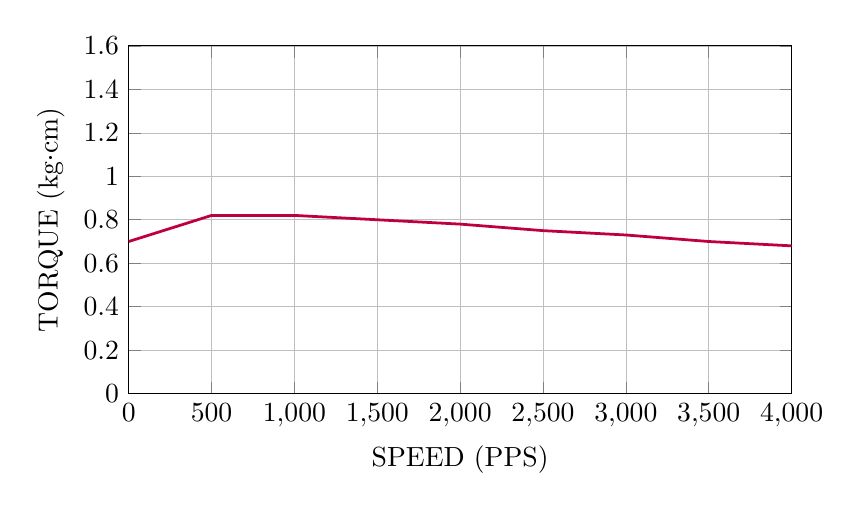
\begin{tikzpicture}
	\begin{axis}[
		width=10cm,
		height=6cm,
		xlabel={SPEED (PPS)},
		ylabel={TORQUE (kg·cm)},
		xmin=0, xmax=4000,
		ymin=0, ymax=1.6,
		xtick={0,500,1000,1500,2000,2500,3000,3500,4000},
		ytick={0,0.2,0.4,0.6,0.8,1,1.2,1.4,1.6},
		legend pos=north east,
		grid=both,
		major grid style={line width=.2pt,draw=gray!50},
		minor grid style={line width=.1pt,draw=gray!20},
		]
		\addplot[
		color=purple,
		line width=1pt
		]
		coordinates {
			(0,0.7)
			(500,0.82)
			(1000,0.82)
			(1500,0.8)
			(2000,0.78)
			(2500,0.75)
			(3000,0.73)
			(3500,0.7)
			(4000,0.68)
		};
	\end{axis}
\end{tikzpicture}